\documentclass{article}

\usepackage[utf8]{inputenc}
\usepackage[danish]{babel}
\usepackage{graphicx}

\title{Analysedokument}
\author{Henrik Romby Mikkelsen og Jacob Scherffenberg-Møller}

\begin{document}

\maketitle
\tableofcontents
\pagebreak

\section{Opgaven}

\subsection{Formål}

Skou Gruppen A/S er en større tømrer/murer-virksomhed, der har omkring 100 ansatte. De har på nuværende tidspunkt ingen kontrol med deres værktøj. Opgaven består i at udvikle et system til intern brug i Skou Gruppen, hvis formål er at skabe kontrol med vikrsomhedens værktøj. Dette gøres ved at registrere hvilke medarbejdere, der er i besiddelse af hvilket værktøj. Systemet vil endvidere medvirke til vedligeholdelse af værktøjet, ved at informere den enkelte ansatte om, at han er i besiddelse af et værktøj, der inden for en given tidshorisont skal til service.

\subsection{Systemdefinition}

Systemets hovedvægt vil ligge på administration og kontrol af værktøj, der skal hjælpe firmaets ledelse med at holde overblik over hvilke ansatte, der har hvilket værktøj. Sekundært vil systemet, også skabe et samlet overblik over alt værktøj firmaet er i besiddelse af. Systemet udvikles som en webapplikation og vil derfor kunne tilgås fra de mest gængse platforme som Mac OS, Windows, Linux og forskellige smartphone-styresystemer. Systemet skal med lethed kunne bruges af folk med begrænsede IT-kundskaber.

\begin{figure}[htbp]
\begin{tabular}{ l p{8cm} }
\hline
Betingelser & Systemet skal kunne bruges af personer med begrænsede IT-kundskaber, hovedsageligt murere og tømrere, men også af kontoruddannede. \\
Anvendelsesområde & Firmaets ledelse -- eventuelt en lageransvarlig til administration af værktøj. Øvrigt ansatte til booking.  \\
Teknologi & Mac OS, Windows, Linux og smartphone-styresystemer. \\
Objekter & Ansatte og værktøj. \\
Funktionalitet & Adminstration og service af værktøj.  \\
Filosofi & Adminstrativt værktøj. \\
\hline
\end{tabular}
\caption{BATOFF}
\end{figure}
\subsection{Omgivelser}

\subsubsection{Problemområde}

Systemet skal registrere alt firmaets værktøj og alle ansatte. For værktøjet er det essentielt at holde styr på, hvilken ansat der er i besiddelse af det, og hvornår det skal til service, så den ansatte kan blive informeret om dette. 

For ansatte er det vigtigste at have en oversigt over alt værktøj, en given ansat er i besiddelse af, så ledelsen til en hver tid kan se, hvad de ansatte har af værktøj. 

\begin{figure}[htbp]
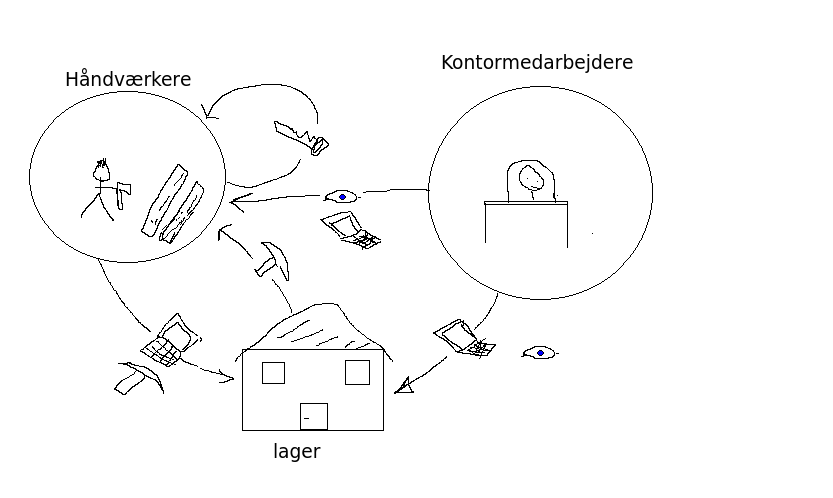
\includegraphics[scale=0.75]{./figures/systemomgivelser.png}
\end{figure}

\subsubsection{Anvendelsesområde}

Systemet skal lette ledelsens arbejdsopgaver omkring kontrol med og administration af firmaets værktøj, og de enkelte ansattes overblik over hvilket værktøj de har ansvar for. 

Ledelsen har mulighed for at indkøbe nyt værktøj og kassere værktøj, der af den ene eller anden grund er blevet ubrugeligt, og ansætte eller afskedige personer.

De ansatte er ikke så central en del af anvendelsesområdet. De skal i grunden kun have mulighed for at aflevere og modtage udleveret værktøj.

\section{Problemområdet}

\subsection{Klynger}

Systemet udvikles med tre klynger: værktøj, begivenheder og personer. Klyngen \emph{værktøj} beskriver en række klasser, der har med værktøj at gøre: værktøjskategori, værktøjsmodel og værktøj. Forholdet mellem disse tre klasser er beskrevet længere nede.

Klyngen \emph{begivenheder} omfatter forskellige klasser, der beskriver en begivenhed i et stykke værktøjs livscyklus. Disse omfatter oprettelse, udlån, servicering, reparation og kassering. Nærmere beskrivelser findes i sektionen \emph{Klasser}.

Klyngen \emph{personer} omfatter en enkelt klasse, brugere. Brugerne registreres med personlige oplysninger samt forskellige parametre i systemet. En mere deltaljeret beskrivelse af klassen \emph{bruger} findes i klassebeskrivelserne nedenfor.

Klyngerne giver en god meta-forståelse af systemets nytte: \emph{værktøj} knyttes sammen med \emph{brugere} gennem forskellige \emph{begivenheder}.

\subsection{Struktur}

Værktøj kan inddeles i forskellige modeller og forskellige kategorier. Strukturen af klyngen \emph{værktøj} er altså to aggregeringer: en fra værktøj til værktøjsmodel, og en fra værktøjsmodel til værktøjskategori. På den måde kommer en værktøjskategori til at indeholde en række værktøjsmodeller, og gennem modellerne også en række værktøj.

Strukturen af klyngen \emph{begivenheder} består af en abstrakt baseklasse samt fem andre klasser, der alle nedarver fra den abstrakte baseklasse -- de indgår i en generaliseringsstruktur. På den måde opnås en abstrakt samling af forskellige begivenheder, der alle på samme måde kan knyttes til et stykke værktøj.

Klyngen \emph{personer} består udelukkende af klassen \emph{bruger}, og der er derfor ikke nogen strukturer internt i denne klynge, der behøver forklaring.

På tværs af klyngerne findes der også en række associationer: en person aggregerer en række begivenheder, således at en person ender med at have en gruppe af begivenheder tilknyttet. Tilknytningen til en begivenhed af underklassen \emph{udlån} vil ligeledes knytte personen til en række værktøj, han er eller har været i besiddelse af.

Værktøj og begivenheder er naturligvis også knyttet sammen i en aggregering, således at et værktøj aggregerer en række begivenheder i løbet af sin levetid. På den måde er det muligt at konstruere en samlet livsbeskrivelse for et stykke værktøj, ligesom det er muligt at lave statistik på værktøjs livsforløb -- for eksempel gennemsnitlig levetid, gennemsnitlig antal service, gennemsnitlig antal reparationer med videre.

\subsection{Klasser}

Værktøjsklyngen udgøres af tre klasser:

\begin{description}

\item[Værktøjskategori] beskriver en mængde værktøj af samme slags -- for eksempel \emph{hammere}, \emph{skruetrækkere} og \emph{save}.

\item[Værktøjsmodel] beskriver en mængde værktøj af samme model -- for eksempel \emph{Black and Decker GT6026} eller \emph{DeWalt DCD710N}. Værktøjsmodellerne knytter sig mange-til-en til værktøjskategorierne, således at kategorierne indeholder en række forskellige værktøjsmodeller.

\item[Værktøj] beskriver et specifikt stykke værktøj, der identificeres ved et nummer eller en unik kode. Værktøjet knytter sig mange-til-en til værktøjstyperne, således at værktøjsmodellerne indeholder alle de stykker værktøj, der er af samme model. På samme måde indeholder værktøjskategorierne alle de stykker værktøj, der er i samme kategori, gennem værktøjsmodel-klassen.

\end{description}

Begivenhedsklyngen udgøres af en abstrakt baseklasse samt fem forskelige specifikke begivenhedsklasser, der alle nedarver fra den abstrakte baseklasse.

\begin{description}

\item[Begivenhed] beskriver en abstrakt begivenhed knyttet til et stykke værktøjs livsforløb. Begivenheden noteres med dato og bruger.

\item[Oprettelse] nedarver fra \emph{begivenhed}, men knytter ikke andre informationer til begivenheden. Denne begivenhedsklasse instantieres hver gang et nyt stykke værktøj oprettes.

\item[Udlån] nedarver ligeledes fra \emph{begivenhed}, og beskriver et udlån til en håndværker. Udlånet registreres med en afslutningsdato, når det afleveres.

\item[Service] beskriver en servicering af et stykke værktøj. Denne klasser nedarver som alle de andre specifikke begivenhedsklasser fra \emph{begivenhed}.

\item[Reparation] beskriver en reparation af et stykke værktøj, hvis det skulle gå i stykker. Reparationen noteres eventuelt med reparatør og med slutdato, idet en reparation kan strække sig over flere dage.

\item[Kassering] beskriver en begivenhed hvor et stykke værktøj kasseres. Den knytter ikke andre informationer til begivenheden, ligesom \emph{oprettelse}.

\end{description}

\begin{figure}[htbp]
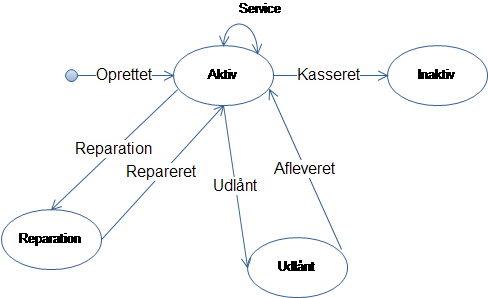
\includegraphics[scale=0.75]{./figures/VTDiag.png}
\end{figure}

Personklyngen består af en enkelt klasse.

\begin{description}

\item[Bruger] beskriver både en bruger i systemet, samt en håndværker i anvendelsesområdet. En bruger registreres med forskellige personlige oplysninger, der skal til for kunne identificere ham. En bruger knyttes til forskellige stykker værktøj, han låner gennem sin ansættelse som håndværker i firmaet, gennem forskellige begivenheder.

\end{description}

\begin{figure}[htbp]
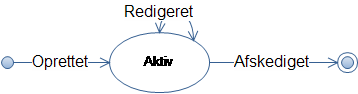
\includegraphics[scale=0.75]{./figures/AnsatTilstandsdiagram.png}
\end{figure}

\subsection{Hændelser}

Nedenfor ses en figur der viser brugsmønstrene for systemets aktører. 

\begin{tabular}{p{4cm} c c}
\hline
{\bf Brugsmønster} & {\bf Kontormedarbejder} & {\bf Håndværker} \\
\hline
Udlån værktøj & X & \\
Aflever værktøj & X & X \\
Overflyt værktøj & X & X \\
Opret værktøj & X & \\
Deaktiver værktøj & X & \\
Ændr værktøj & X & \\
Servicer værktøj & X & \\
Reparer værktøj & X & \\
Opret ansat & X & \\
Deaktiver ansat & X & \\
Ændr ansat & X & \\
\end{tabular}
\section{Anvendelsesområdet}

\subsection{Brug}

\subsubsection{Oversigt}
Vi har identificeret 2 aktører, Kontormedarbjedere og Håndværkerer og i alt 10 brugsmønstre, se tabellen ovenfor. 
\subsubsection{Aktører}

Figuren nedenfor viser de to roller, der er identificeret i systemet.

\begin{tabular}{p{5cm} p{5cm}}
\hline
{\bf Kontormedarbejder} & {\bf Håndværker} \\
\hline
\emph{Formål} En ansat i firmaets administrationsafdeling, der tager sig af de daglige kontormæssige arbejdsopgaver & \emph{Formål} En medarbejder, der arbejder \emph{ude i marken}. Han benytter det værktøj, der er registreret i systemet. \\
\emph{Karakteristik} Udføres af personer med mere eller mindre erfaring i kontorarbejde. En vis IT-erfaring forventes & \emph{Karakteristik} Udføres af håndværkere med forskellig uddannelses- og erhverserfaring. Mange vil have IT-erfaring, men det kan ikke forventes. \\

\emph{Eksempler} En kontoruddannet person, der er fastansat til at tage sig af administrative opgaver. Stor IT-erfaring i forbindelse med de administrative opgaver.

En person under uddannelse, der hjælper til med administrative opgaver som del af et praktikforløb. Forholdsvist stor IT-erfaring fra uddannelse og internetsurfing. & \emph{Eksempler} En håndværker-mester, der udfører håndværkerarbejde forskellige steder i løbet af en dag, med eller uden andre håndværkere. Har ikke større IT-erfaring end at han kan benytte Word og lignende.

En lærling, der følger en mester rundt på forskellige opgaver. Har IT-erfaring fra generelt internetforbrug.
\end{tabular}

\subsubsection{Brugsmønstre}

Brugsmønstrene kan inddeles i forskellige grupper.
\begin{itemize}
\item Opret Værktøj/Ansat
\item Deaktiver Værktøj/Ansat
\item Ændr Værktøj/Ansat
\end{itemize} 
Brugsmønstrene opdaterer alle modellen med nye eller ændrede informationer om en ansat, en gruppe af værktøj eller et specifikt stykke værktøj.

\begin{tabular}{p{10cm}}
\hline
\centerline{Opret værktøj}\\
\hline
\emph{Mønster:} Brugsmønsteret er aktuelt, nå nyt værktøj er blevet indkøbt, værktøjet oprettets under en kategori og model, om det nye værktøj registres indkøbspris, et navn.\\ 
\hline
\end{tabular}


\begin{itemize}
\item Udlån \& Aflever værktøj \& Overflyt værktøj
\end{itemize} 
Et specifikt stykke værktøj udlånes til en medarbejder, der er registreret i systemet, nå han ikke længere bruger det, afleveres det. 


\begin{tabular}{p{10cm}}
\hline
\centerline{Udlån værktøj}\\
\hline
\emph{Mønster:} Værktøjet er på lager og en håndværker skal bruge det, han fortager et lån i systemet og værktøjet registreres, som værende udlånt til den medarbejder, som foretager lånet.\\
\hline
\end{tabular}


\begin{tabular}{p{10cm}}
\hline
\centerline{Overflyt værktøj}\\
\hline
\emph{Mønster:} Et givent værktøj er udlånt til en medarbejder, en anden medarbejder låner værktøjet til en opgave og tager det efterfølgende med sig, de to medarbejdere skal så registrere en overflytning i systemet, så det kan ses at den anden medarbejder nu er i besiddelse af værktøjet.\\
\hline  
\end{tabular}


\begin{itemize}
\item Servicer \& Reparer
\end{itemize} 
Værktøj skal med jævne mellemrum til service, service intervalerne er indlejret i systemet. Endvidere er der en åbenlys risiko for defekt, som skal udbedres ved en reparation. 

\subsection{Funktioner}

\subsubsection{Komplet funktionsliste}

Nedenfor ses en figur, der opridser systemets understøttede funktioner.

\begin{tabular}{p{5cm} p{2.5cm} p{2.5cm}}
\hline
{\bf Funktion} & {\bf Kompleksitet} & {\bf Type} \\
\hline
Opret, ændr, deaktiver værktøj & Simpel & Opdatering \\
Opret, ændr, deaktiver ansat & Simpel & Opdatering \\
Udlån, aflever, overflyt værktøj & Simpel & Opdatering \\
Servicer, reparer værktøj & Simpel & Opdatering \\
Hjemkald værktøj (SMS) & Kompleks & Signalering \\
Fremvis værktøj/ansat & Simpel & Aflæsning \\
\end{tabular}

\subsection{Brugergrænsefladen}
Brugergrænsefladen er på dansk, og der bruges derfor danske termer i alle dele af grænsefladen, nedenfor ses et udsnit af vores brugergrænsefladedesign.

\subsubsection{Dialogform}
Brugergrænsefladen består af en menu i toppen af billedet, som altid er tilstede så man altid kan navigerer, hvorhen i systemet det skal være uanset, hvor man er endt. 
Forsiden består af en række kasser, der indeholder hurtig adgang, til de primære opgaver for, de forskellige aktører. Dette er den mest overskuelige løsning, og vil ligne noget bruger er stødt på i andre programmer, hvilket vil lette tilvæningen til det nye system.

\begin{figure}[htbp]
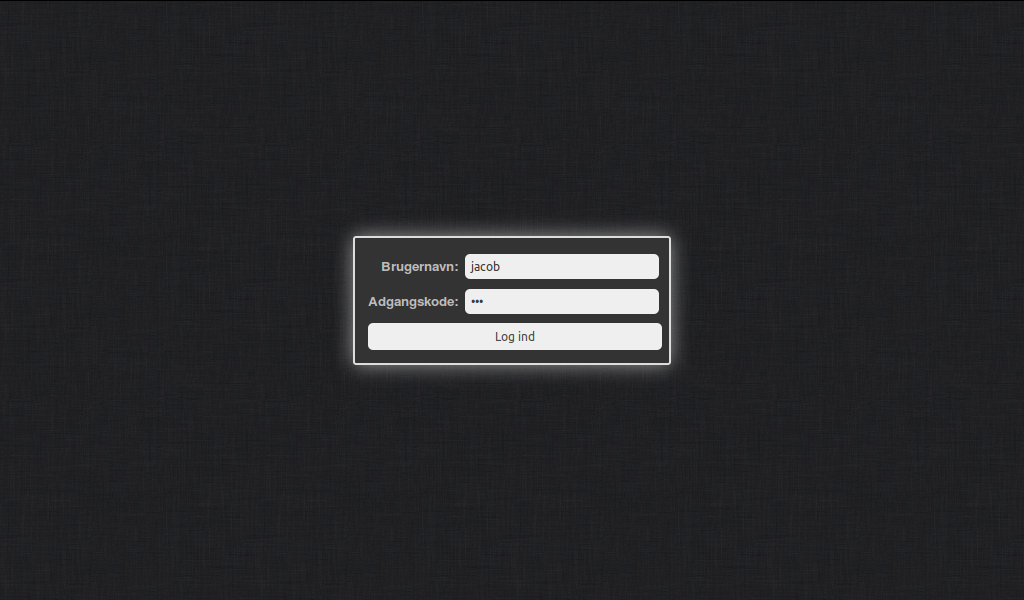
\includegraphics[scale=0.40]{./figures/loginpage.png}
\end{figure}

\begin{figure}[htbp]
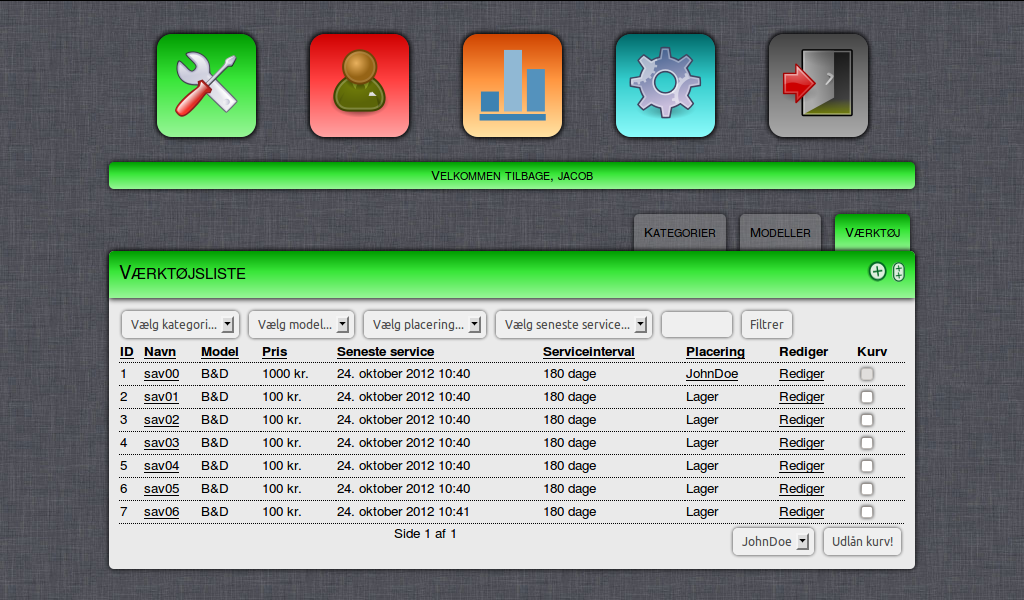
\includegraphics[scale=0.40]{./figures/tools.png}
\end{figure}

\begin{figure}[htbp]
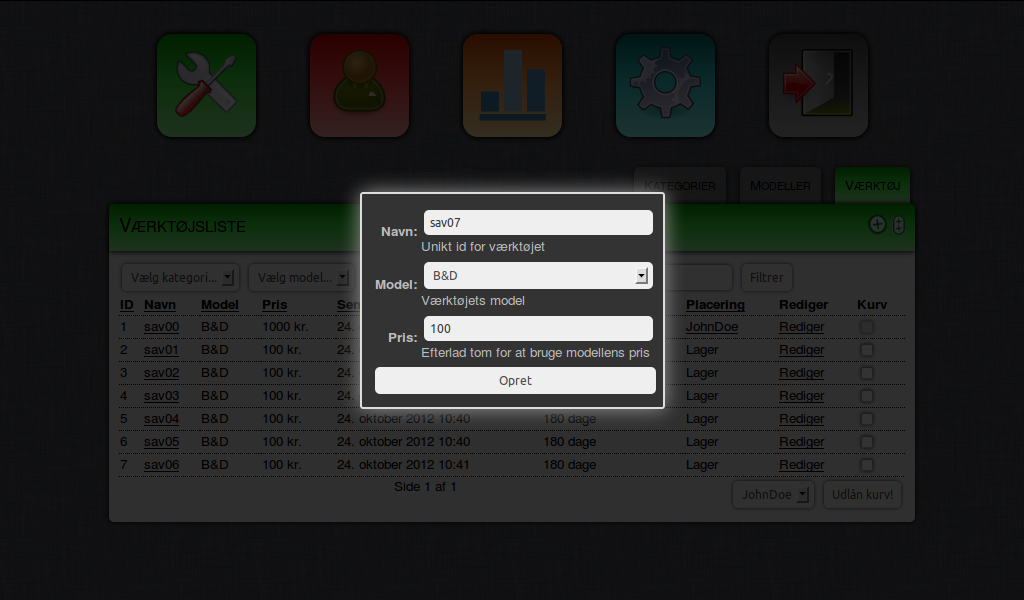
\includegraphics[scale=0.40]{./figures/createtool.png}
\end{figure}

\begin{figure}[htbp]
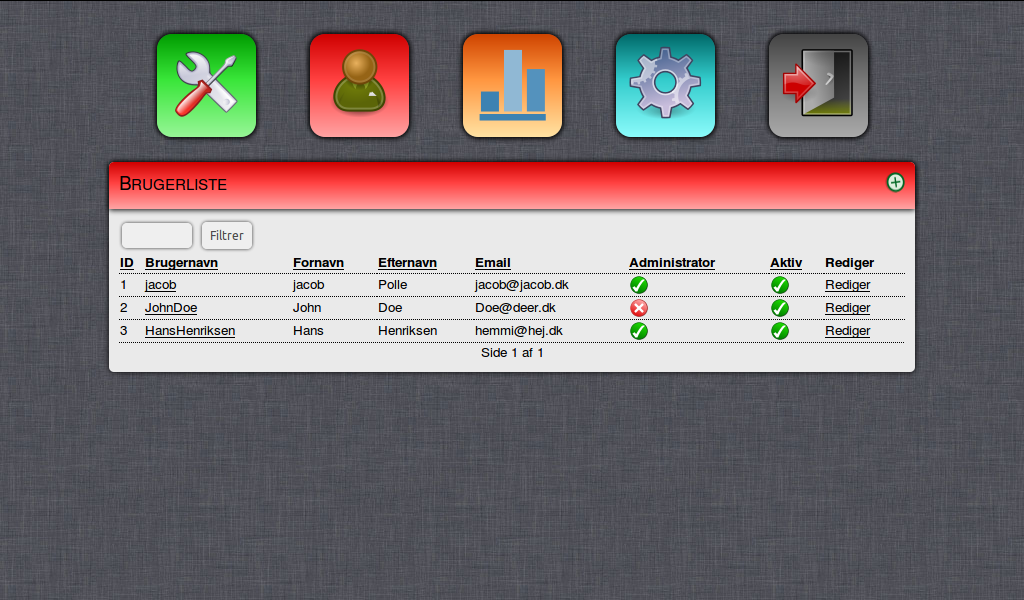
\includegraphics[scale=0.40]{./figures/Users.png}
\end{figure}

 
\subsection{Den tekniske platform}

Systemet udvikles som en webapplikation i Python-frameworket Django. Ved at udvikle en webapplikation virker systemet på det bredest mulige spektrum af styresystemer, idet alle datamater med en browser principielt kan benytte systemet, for eksempel Mac OS, Windows, Linux og smartphone-styresystemer. Systemet skal således kunne styres med både mus og tastatur, og via input fra berøring ved brug af smartphones. 

\section{Anbefalinger}

\subsection{Systemets nytte og realiserbarhed}
Det beskrevne system skal fungere, som en hjælp til at lette de kontoransattes kontrol med værktøj i firmaet, samt give et overblik over, hvor mange penge der er brugt på værktøj i firmaet. Endvidere vil det altid i systemet fremgå, hvor værktøj befinder sig, lager, udlånt, service eller reparation. 
For hånderværkerne vil det give overblik over hvilket værktøj, man er ansvarlig for, og via signalering fra systemet, gøre opmærksom på at man inden for en givne periode, skal have afleveret et stykke værktøj til service. 
Realiserbarheden er meget stor, der er ingen økonomi i systemet, så dette bliver ikke en hæmsko, systemet kan uden større besværligheder, tilrettes kundens ønsker. Kundens entusiamse i at få færdiggjort systemet, øger i vores øjne også realiserbarheden.   

\subsection{Strategi}
Kunden er meget entusiatisk omkring systemet, og har givet udtryk for en stor lyst til at være en del af udviklingen, og være med til at realisere systemet. Planen er at vi laver en grundig analyse af anvendelses- og problemområde (som blandt andet denne rapport er en del af), og først derefter går igang med implementeringen af systemet. På denne måde regner vi med at kunne eliminere en stor del af de problemer, som vi eventuelt ville have stødt på under udviklingsarbejdet.

\end{document}
